% =====================================================================
%  BÁO CÁO: HỢP ĐỒNG NHÓM & GIỚI THIỆU GAME TETRIS
% =====================================================================
\documentclass[12pt,a4paper,oneside]{report}
% Cỡ chữ thân bài cố định 13pt: định nghĩa lại \normalsize để mọi chỗ gọi \normalsize đều ra 13pt
\makeatletter
\renewcommand\normalsize{\@setfontsize\normalsize{13pt}{16pt}}
\makeatother
\usepackage{iftex}
\usepackage{booktabs}
\ifPDFTeX
  \usepackage[utf8]{inputenc}
  \usepackage[T5]{fontenc}
  \usepackage[vietnamese]{babel}
  \usepackage{mathptmx}
\else
  \usepackage{fontspec}
  \setmainfont{texgyretermes}[
    Extension=.otf, UprightFont=*-regular, BoldFont=*-bold,
    ItalicFont=*-italic, BoldItalicFont=*-bolditalic]
\fi

% ---------- Khổ giấy, lề, giãn dòng ----------
\usepackage[a4paper,left=3cm,right=2cm,top=2.5cm,bottom=2.5cm]{geometry}
\usepackage{setspace}
\setstretch{1.3}
\usepackage{parskip}
\setlength{\parskip}{6pt}
\setlength{\parindent}{1cm}
\usepackage{indentfirst}
\sloppy
\hyphenpenalty=10000
\exhyphenpenalty=10000

\usepackage{float}
\usepackage{xcolor}
\usepackage{graphicx}
\usepackage{tikz}
\usepackage{array}
\usepackage{enumitem}
\usepackage{titlesec}
\usepackage{fancyhdr}
\usepackage{xurl}
\usepackage{hyperref}
\hypersetup{
    colorlinks=true,
    citecolor=blue,
    linkcolor=black,   % Giữ màu đen cho mục lục
    urlcolor=blue
}

\setlist{itemsep=0pt,topsep=2pt,leftmargin=1.5cm}

% ---------- Định dạng tiêu đề chương / mục ----------
\titleformat{\chapter}[display]
  {\centering\bfseries\large}{CHƯƠNG \thechapter}{4pt}{\MakeUppercase}
\titlespacing*{\chapter}{0pt}{0pt}{18pt}
\titleformat{\section}{\bfseries\normalsize}{\thesection.}{0.5em}{}
\titleformat{\subsection}{\bfseries\itshape\normalsize}{\thesubsection.}{0.5em}{}

% ---------- Header / footer ----------
\pagestyle{fancy}
\fancyhf{}
\fancyhead[L]{\small Trường ĐH Công nghệ Thông tin -- ĐHQG-HCM}
\fancyhead[R]{\small Báo cáo môn học}
\fancyfoot[C]{\thepage}
\setlength{\headheight}{16pt}
\renewcommand{\headrulewidth}{0.4pt}
\fancypagestyle{plain}{\fancyhf{}\fancyfoot[C]{\thepage}\renewcommand{\headrulewidth}{0pt}}

% ---------- Chữ ký: dùng ảnh nếu có file, không thì để trống ô ký ----------
\newcommand{\chuky}[1]{\IfFileExists{#1}{\includegraphics[height=2cm,width=4cm,keepaspectratio]{#1}}{\rule{0pt}{2cm}}}

\begin{document}

% Đặt lại tên các mục (sau \begin{document} để babel không ghi đè)
\renewcommand{\contentsname}{MỤC LỤC}
\renewcommand{\tablename}{Bảng}
\renewcommand{\bibname}{NGUỒN THAM KHẢO}

% =========================== TRANG BÌA ==============================
\begin{titlepage}
\begin{tikzpicture}[remember picture,overlay]
  \draw[line width=2pt]
    ([xshift=2cm,yshift=-1.5cm]current page.north west)
    rectangle ([xshift=-1.5cm,yshift=1.5cm]current page.south east);
  \draw[line width=0.6pt]
    ([xshift=2.15cm,yshift=-1.65cm]current page.north west)
    rectangle ([xshift=-1.65cm,yshift=1.65cm]current page.south east);
\end{tikzpicture}
\begin{center}
\setstretch{1.2}
{\large ĐẠI HỌC QUỐC GIA THÀNH PHỐ HỒ CHÍ MINH}\\
{\large\bfseries TRƯỜNG ĐẠI HỌC CÔNG NGHỆ THÔNG TIN}\\
{\large\bfseries KHOA KHOA HỌC MÁY TÍNH}\\[2pt]
\rule{6cm}{0.6pt}\\[1cm]

\IfFileExists{imgs/Logo_UIT.jpg}{%
  
\includegraphics[width=4.2cm]{imgs/Logo_UIT.jpg}%
}{%
  \fbox{\parbox[c][3.5cm][c]{3.5cm}{\centering LOGO UIT\\\small(Logo\_UIT.jpg)}}%
}\\[1cm]

{\Large\bfseries BÁO CÁO MÔN HỌC}\\[4pt]
{\large KỸ NĂNG NGHỀ NGHIỆP -- SS004}\\[1.2cm]

{\large\bfseries ĐỀ TÀI:}\\[6pt]
{\LARGE\bfseries HỢP ĐỒNG NHÓM VÀ\\[4pt]
GIỚI THIỆU GAME TETRIS}\\[1.5cm]

\begin{tabular}{ll}
\textbf{Giảng viên hướng dẫn:} & Nguyễn Văn Toàn\\[4pt]
\textbf{Sinh viên thực hiện:}  & Nguyễn Thịnh -- MSSV: 26521929\\
                               & Nguyễn Việt Lâm -- MSSV: 26521077\\
                               & Trương Tấn Phát -- MSSV: 26521563\\
                               & Thái Trí Nhân -- MSSV: 26521457\\
                               & Võ Ngọc Thơ -- MSSV: 25521792\\[4pt]
\textbf{Lớp:}                  & SS004.R11\\
\end{tabular}

\vfill
{\large TP. Hồ Chí Minh, tháng 11 năm 2026}
\end{center}
\end{titlepage}

% =========================== MỤC LỤC ================================
\pagenumbering{roman}
\setcounter{page}{1}
\tableofcontents
\thispagestyle{empty}

% =========================== NỘI DUNG ===============================
\clearpage
\pagenumbering{arabic}
\setcounter{page}{1}

% --------------------------------------------------------------------
%  CHƯƠNG 1 -- Hợp đồng nhóm
% --------------------------------------------------------------------
\chapter{Hợp đồng nhóm}

\section{Tên nhóm: Năm anh em siêu nhân}

\section{Thành viên nhóm}

\begin{table}[H]
\centering
\vspace{-0.8cm}
\caption{Danh sách thành viên nhóm}\label{tab:danh_sach_thanh_vien}
\renewcommand{\arraystretch}{1.2}
\begin{tabular}{|>{\centering\arraybackslash}p{1cm}|>{\raggedright\arraybackslash}p{4.5cm}|>{\raggedright\arraybackslash}p{2.5cm}|>{\raggedright\arraybackslash}p{3.5cm}|}
\hline
\textbf{STT} & \textbf{Họ và tên} & MSSV & \textbf{Vai trò chính} \\ \hline
1 & Nguyễn Thịnh    & 26521929 & Trưởng nhóm \\ \hline
2 & Nguyễn Việt Lâm & 26521077 & Thành viên \\ \hline
3 & Trương Tấn Phát & 26521563 & Thành viên \\ \hline
4 & Thái Trí Nhân   & 26521457 & Thành viên \\ \hline
5 & Võ Ngọc Thơ     & 25521792 & Thành viên \\ \hline
\end{tabular}
\end{table}

\section{Mục tiêu của nhóm}

\begin{itemize}
    \item Hoàn thành đầy đủ các nội dung của bài tập và nộp đúng thời hạn theo yêu cầu của học phần.
    \item Tìm hiểu các phiên bản game Tetris thông dụng để viết phần giới thiệu, hướng dẫn chơi và xác định các chức năng chính, làm cơ sở thiết kế game của nhóm ở các giai đoạn sau.
    \item Thống nhất cách làm việc, phân công rõ trách nhiệm và bảo đảm mỗi thành viên đều có phần việc cụ thể.
    \item Sử dụng hiệu quả các công cụ làm việc nhóm như Slack, Trello, GitHub và Overleaf để trao đổi, quản lý tiến độ, quản lý mã nguồn và biên soạn tài liệu.
    \item Rèn luyện kỹ năng giao tiếp, phối hợp, giải quyết vấn đề, quản lý thời gian và chịu trách nhiệm với phần việc được giao.
\end{itemize}

\section{Nội dung báo cáo}

Báo cáo của nhóm gồm các phần sau:
\begin{enumerate}[leftmargin=1.5cm]
    \item \textbf{Hợp đồng nhóm:} thành viên, mục tiêu, phân công, công cụ làm việc, quy định, tiêu chí đánh giá và chữ ký của tất cả thành viên.
    \item \textbf{Các link công cụ nhóm sử dụng:} Slack, Trello, GitHub, Overleaf. Repository GitHub chỉ chứa code khởi tạo của game Tetris do giảng viên cung cấp.
    \item \textbf{Giới thiệu và hướng dẫn chơi game Tetris:} dựa trên các phiên bản Tetris thông dụng, trình bày game này ra sao, cách chơi dành cho người dùng cuối và các chức năng chính. Độ dài từ 2 đến 10 trang, viết hấp dẫn, dễ hiểu.
    \item \textbf{Đánh giá thực hiện hợp đồng nhóm:} đánh giá từng thành viên theo tiêu chí ở mục~\ref{sec:tieu_chi}.
\end{enumerate}

\section{Phân công nhiệm vụ}

\begin{table}[H]
\centering
\vspace{-0.8cm}
\caption{Phân công nhiệm vụ các thành viên}\label{tab:phan_cong_nhiem_vu}
\renewcommand{\arraystretch}{1.45}
\begin{tabular}{|>{\raggedright}p{3.4cm}|>{\raggedright\arraybackslash}p{9.2cm}|}
\hline
\textbf{Thành viên} & \textbf{Nhiệm vụ} \\ \hline
Nguyễn Thịnh &
Trưởng nhóm: phân công công việc, theo dõi tiến độ trên Trello; quản lý repository GitHub; biên soạn hợp đồng nhóm; nhận file \texttt{.tex} của các thành viên và đồng bộ vào Overleaf; đồng bộ bản cuối cùng lên GitHub.
\\ \hline
Nguyễn Việt Lâm &
Viết phần giới thiệu game Tetris: lịch sử, ý tưởng game này ra sao.
\\ \hline
Trương Tấn Phát &
Rà soát toàn bộ báo cáo: kiểm tra chính tả, định dạng thống nhất giữa các phần và nguồn tham khảo.
\\ \hline
Thái Trí Nhân &
Viết phần cách chơi dành cho người dùng cuối: luật chơi, phím điều khiển, cách tính điểm, cấp độ, điều kiện thua.
\\ \hline
Võ Ngọc Thơ &
Viết phần các chức năng chính của game; vẽ hình minh họa các chức năng.
\\ \hline
\end{tabular}
\end{table}

\textbf{Thời hạn chung:} hoàn thành toàn bộ báo cáo trước 23:59 ngày 11/11/2026.

Overleaf là bản chính của báo cáo (do Overleaf giới hạn số người được chỉnh sửa, các thành viên khác chỉ có quyền xem). Mỗi thành viên sau khi hoàn thành phần việc của mình gửi file \texttt{.tex} của phần đó qua Slack cho trưởng nhóm để đồng bộ vào Overleaf. File \texttt{hop\_dong\_nhom.tex} trên GitHub chỉ được đồng bộ một lần khi báo cáo hoàn tất.

\section{Công cụ và không gian làm việc nhóm}

Nhóm sử dụng các công cụ/không gian trực tuyến để trao đổi, quản lý công việc, quản lý mã nguồn và biên soạn tài liệu.

\begin{table}[H]
\centering
\caption{Danh sách công cụ và không gian làm việc nhóm}\label{tab:cong_cu_lam_viec}
\renewcommand{\arraystretch}{1.55}
\begin{tabular}{|>{\raggedright\arraybackslash}p{2.5cm}|>{\raggedright\arraybackslash}p{6.2cm}|>{\raggedright\arraybackslash}p{5.5cm}|}
\hline
\textbf{Công cụ} & \textbf{Mục đích sử dụng} & \textbf{Link} \\ \hline
\textbf{Slack} &
Kênh trao đổi chính của nhóm; trao đổi công việc, thông báo và giải quyết thắc mắc &
\url{https://app.slack.com/client/T0BV8JTK6QH/C0CFTHSUY5C} \\ \hline
\textbf{Trello} &
Phân công nhiệm vụ, theo dõi trạng thái công việc và tiến độ &
\url{https://trello.com/invite/b/6af011e459b2a704ab3a241d/ATTI8d77df4ce00143fb38765a5affeeefc69B915E21/tetris} \\ \hline
\textbf{GitHub} &
Quản lý mã nguồn game Tetris (hiện chỉ có code khởi tạo do giảng viên cung cấp); lưu bản báo cáo cuối cùng &
\url{https://github.com/26521929-Nguyen-Thinh/The-tetris} \\ \hline
\textbf{Overleaf} &
Bản chính của báo cáo (LaTeX); trưởng nhóm chỉnh sửa, các thành viên xem và góp ý &
\url{https://www.overleaf.com/project/6af006b50925752415376809/share#0d2864ee799ce7b692dc5eb9b5288f7eee1bafbbcddd25bc} \\ \hline
\end{tabular}
\end{table}

\section{Quy định làm việc}

\begin{itemize}
    \item Mọi trao đổi chính thức thực hiện trên Slack; thành viên phản hồi tin nhắn của nhóm trong vòng 24 giờ.
    \item Mỗi nhiệm vụ được tạo thành thẻ trên Trello, có người phụ trách và hạn hoàn thành; thành viên tự cập nhật trạng thái thẻ.
    \item Mỗi thành viên gửi file \texttt{.tex} phần việc của mình qua Slack cho trưởng nhóm; trưởng nhóm đồng bộ vào Overleaf để cả nhóm rà soát. Góp ý cho phần của người khác gửi trên Slack, không tự sửa.
    \item Quyết định chung được thông qua theo đa số; nếu không thống nhất, trưởng nhóm quyết định cuối cùng.
    \item Thành viên trễ hạn phải báo trước cho nhóm. Trễ hạn nhiều lần hoặc không đóng góp sẽ được ghi nhận trong phần đánh giá và báo cáo với giảng viên.
\end{itemize}

\section{Tiêu chí đánh giá hợp tác nhóm}\label{sec:tieu_chi}

\begin{table}[H]
\centering
\small
\vspace{-0.8cm}
\caption{Tiêu chí đánh giá hợp tác nhóm}\label{tab:rubric_danh_gia}
\renewcommand{\arraystretch}{1.3}
\begin{tabular}{|>{\raggedright}p{2.4cm}|*{4}{>{\raggedright\arraybackslash}p{2.8cm}|}}
\hline
\textbf{Tiêu chí} &
\textbf{4 -- Xuất sắc} &
\textbf{3 -- Tốt} &
\textbf{2 -- Đạt} &
\textbf{1 -- Chưa đạt} \\ \hline
Thái độ &
Luôn tích cực, tôn trọng và hỗ trợ thành viên khác. &
Thái độ tích cực, không phát sinh vấn đề. &
Thái độ tích cực, nhưng đôi lúc cần nhắc nhở. &
Thái độ tiêu cực, gây ảnh hưởng đến hoạt động nhóm. \\ \hline
Đóng góp &
Chủ động đưa ra ý tưởng, hoàn thành nhiệm vụ vượt yêu cầu. &
Có đóng góp và hoàn thành nhiệm vụ. &
Có đóng góp nhưng đôi lúc cần nhắc nhở. &
Không đóng góp. \\ \hline
Quản lý thời gian &
Hoàn thành nhiệm vụ trước thời hạn. &
Hoàn thành nhiệm vụ đúng thời hạn. &
Hoàn thành nhiệm vụ đúng thời hạn nhưng đôi lúc chậm hoặc cần hỗ trợ. &
Không hoàn thành hoặc trễ hạn nhiều lần. \\ \hline
Đóng góp ý kiến &
Chủ động đưa ra ý kiến. &
Đưa ra ý kiến khi cần thiết. &
Chỉ đưa ra ý kiến khi được hỏi. &
Không đưa ra ý kiến cho nhóm. \\ \hline
Làm việc nhóm &
Luôn lắng nghe, đóng góp, hỗ trợ các thành viên khác trong quá trình làm việc nhóm. &
Luôn tham gia làm việc nhóm. &
Có tham gia làm việc nhóm. &
Không tham gia làm việc nhóm, gây ảnh hưởng đến hoạt động của nhóm. \\ \hline
\end{tabular}
\end{table}

\section{Cam kết của nhóm}

Chúng tôi thống nhất các nội dung trên và cam kết phối hợp, hoàn thành phần việc được giao, tôn trọng quyết định chung và cùng chịu trách nhiệm về sản phẩm cuối cùng của nhóm.

% Ảnh chữ ký đặt trong imgs/chu_ky/: thinh.png, lam.png, phat.png, nhan.png, tho.png
\vspace{8pt}
\begin{center}
\renewcommand{\arraystretch}{1.5}
\begin{tabular}{ccc}
\textbf{Trưởng nhóm} & \textbf{Thành viên} & \textbf{Thành viên}\\
\textit{(Ký, ghi rõ họ tên)} & \textit{(Ký, ghi rõ họ tên)} & \textit{(Ký, ghi rõ họ tên)} \\
\chuky{imgs/chu_ky/thinh.png} & \chuky{imgs/chu_ky/lam.png} & \chuky{imgs/chu_ky/phat.png} \\
\textbf{Nguyễn Thịnh} & \textbf{Nguyễn Việt Lâm} & \textbf{Trương Tấn Phát}\\[16pt]
\end{tabular}

\begin{tabular}{cc}
\textbf{Thành viên} & \textbf{Thành viên}\\
\textit{(Ký, ghi rõ họ tên)} & (Ký, ghi rõ họ tên) \\
\chuky{imgs/chu_ky/nhan.png} & \chuky{imgs/chu_ky/tho.png} \\
\textbf{Thái Trí Nhân} & \textbf{Võ Ngọc Thơ}\\
\end{tabular}
\end{center}

% --------------------------------------------------------------------
%  CHƯƠNG 2 -- Giới thiệu và hướng dẫn chơi game Tetris (2--10 trang)
% --------------------------------------------------------------------
\chapter{Giới thiệu và hướng dẫn chơi game Tetris}


\section{Giới thiệu game Tetris}
% =====================================================================
%  PHẦN: GIỚI THIỆU GAME TETRIS (lịch sử, ý tưởng game)
%  Người viết: Nguyễn Việt Lâm
% =====================================================================

\providecommand{\khoitetromino}[2]{%
  \foreach \x/\y in {#1}{%
    \draw[fill=black!#2,line width=0.6pt] (\x*0.5,\y*0.5) rectangle ++(0.5,0.5);}}

\subsection{Lịch sử ra đời}

Tetris là một trò chơi xếp hình ra đời tại Moscow, Liên Xô, vào giữa thập niên 1980. Tác giả của game là Alexey Pajitnov, một kỹ sư phần mềm làm việc tại Trung tâm Tính toán thuộc Viện Hàn lâm Khoa học Liên Xô, chuyên nghiên cứu về nhận dạng giọng nói. Ngoài giờ làm việc, ông thường viết những trò chơi nhỏ trên chiếc máy tính Elektronika 60 của viện để thử khả năng của máy, đồng thời để mọi người xung quanh có thêm niềm vui~\cite{tetris_wiki,tetris_myjoy}.

Ý tưởng của Tetris xuất phát từ một món đồ chơi thời thơ ấu của Pajitnov: bộ xếp hình \textit{pentomino}. Trong bộ đồ chơi này, người chơi phải sắp xếp 12 mảnh ghép, mỗi mảnh được tạo từ 5 ô vuông, vào vừa khít một chiếc hộp. Vào tháng 6 năm 1984, ông nảy ra ý định đưa trò xếp hình này lên máy tính. Tuy nhiên, việc cho 12 loại mảnh ghép xoay và rơi theo thời gian thực quá phức tạp, nên ông rút gọn lại còn các mảnh ghép chỉ gồm 4 ô vuông, gọi là \textit{tetromino}~\cite{guardian_tetris,tetris_wiki}. Cái tên \textit{Tetris} được ghép từ ``\textit{tetra}'' (tiếng Hy Lạp nghĩa là bốn) và ``\textit{tennis}'' (môn thể thao yêu thích của tác giả)~\cite{filfre_tetris}.

Phiên bản đầu tiên rất đơn sơ. Chiếc Elektronika 60 chỉ hiển thị được chữ, không có đồ họa, nên các khối gạch phải được vẽ bằng những ký tự như dấu ngoặc vuông. Dù vậy, game nhanh chóng khiến các đồng nghiệp của Pajitnov mê mẩn, ai chơi thử cũng khó rời máy. Sau đó, với sự giúp đỡ của Dmitry Pavlovsky và Vadim Gerasimov, Tetris được chuyển sang máy tính IBM PC phổ biến hơn. Trò chơi lan truyền trong giới lập trình viên chủ yếu qua việc chép lại trên đĩa mềm và truyền miệng, rồi dần ra khỏi biên giới Liên Xô~\cite{denofgeek_tetris,tetris_myjoy}.

Sau nhiều năm tranh chấp bản quyền phức tạp, Tetris được phát hành ở phương Tây và nổi tiếng toàn cầu nhất là nhờ bản Game Boy của Nintendo năm 1989. Đến năm 1996, quyền sở hữu game trở về tay Pajitnov; ông cùng Henk Rogers thành lập The Tetris Company để quản lý việc cấp phép cho các phiên bản chính thức~\cite{tetris_wiki,tetris_myjoy}. Cho đến nay, Tetris đã xuất hiện trên hơn 65 nền tảng khác nhau và có hơn nửa tỷ lượt tải trên thiết bị di động, theo thống kê của The Tetris Company~\cite{tetris_myjoy}.

\subsection{Ý tưởng của game}

Ý tưởng của Tetris đơn giản đến mức chỉ cần xem vài giây là hiểu: các khối gạch rơi dần xuống từ phía trên màn hình, người chơi xoay và di chuyển chúng để xếp thành những hàng ngang kín, không còn khoảng trống. Mỗi hàng kín sẽ biến mất và người chơi được cộng điểm. Nếu các khối chất cao chạm tới đỉnh màn hình thì trò chơi kết thúc.

Mọi khối gạch trong Tetris đều là \textit{tetromino}, tức hình được ghép từ đúng 4 ô vuông nối với nhau theo cạnh. Với cách ghép này chỉ có 7 hình dạng khác nhau, thường được gọi theo hình dáng của chúng là I, O, T, S, Z, J và L (Hình~\ref{fig:bay_tetromino}). Trong bản tiêu chuẩn hiện nay, khu vực chơi là một cột dọc rộng 10 ô và cao 20 ô.

\begin{figure}[H]
\centering
\begin{tikzpicture}[scale=0.95]
  \begin{scope}[shift={(0,0)}]
    \khoitetromino{0/0,1/0,2/0,3/0}{10}
    \node at (1,-0.45) {I};
  \end{scope}
  \begin{scope}[shift={(2.6,0)}]
    \khoitetromino{0/0,1/0,0/1,1/1}{25}
    \node at (0.5,-0.45) {O};
  \end{scope}
  \begin{scope}[shift={(4.2,0)}]
    \khoitetromino{0/0,1/0,2/0,1/1}{40}
    \node at (0.75,-0.45) {T};
  \end{scope}
  \begin{scope}[shift={(6.4,0)}]
    \khoitetromino{1/0,2/0,0/1,1/1}{15}
    \node at (0.75,-0.45) {S};
  \end{scope}
  \begin{scope}[shift={(8.6,0)}]
    \khoitetromino{0/0,1/0,1/1,2/1}{30}
    \node at (0.75,-0.45) {Z};
  \end{scope}
  \begin{scope}[shift={(10.8,0)}]
    \khoitetromino{0/0,1/0,2/0,0/1}{20}
    \node at (0.75,-0.45) {J};
  \end{scope}
  \begin{scope}[shift={(13.0,0)}]
    \khoitetromino{0/0,1/0,2/0,2/1}{35}
    \node at (0.75,-0.45) {L};
  \end{scope}
\end{tikzpicture}
\caption{Bảy khối tetromino trong game Tetris}\label{fig:bay_tetromino}
\end{figure}

Sức hấp dẫn của Tetris nằm ở chỗ luật chơi rất ít nhưng tình huống thì gần như không lặp lại. Các khối xuất hiện ngẫu nhiên, nên mỗi lượt người chơi phải quan sát nhanh, quyết định đặt khối vào đâu và xoay theo hướng nào sao cho không để lại các lỗ trống khó lấp. Khi trò chơi tiến triển, các khối rơi nhanh hơn, tạo ra áp lực tăng dần: chơi giỏi hơn thì càng được thử thách nhiều hơn. Chính sự kết hợp giữa luật chơi dễ học, tốc độ tăng dần và cảm giác thỏa mãn mỗi khi một hàng biến mất khiến Tetris dễ chơi nhưng khó dừng~\cite{filfre_tetris}.

\subsection{Sức ảnh hưởng của Tetris}

Hơn bốn thập kỷ sau khi ra đời, Tetris vẫn được xem là một trong những trò chơi điện tử nổi tiếng và được chơi rộng rãi nhất thế giới. Game có mặt trên máy tính, máy chơi game cầm tay, máy console và điện thoại thông minh, được người chơi ở mọi lứa tuổi yêu thích. Sự thành công này cho thấy một ý tưởng đơn giản, được thiết kế khéo, có thể tồn tại lâu hơn nhiều so với những trò chơi dùng đồ họa và công nghệ phức tạp.

Với nhóm chúng tôi, đây cũng là lý do Tetris là một đề tài phù hợp: luật chơi rõ ràng, dễ hình dung, nhưng khi lập trình lại chứa nhiều bài toán thú vị như điều khiển khối rơi, xoay khối, kiểm tra va chạm và xóa hàng. Phần giới thiệu này là nền tảng để các phần tiếp theo trình bày cách chơi và các chức năng chính mà game của nhóm hướng tới.


\section{Cách chơi}
% =====================================================================
%  PHẦN: CÁCH CHƠI (luật chơi, phím điều khiển, tính điểm, cấp độ, điều kiện thua)
%  Người viết: Thái Trí Nhân
% =====================================================================

Tetris là một trong số ít trò chơi mà bạn có thể hiểu luật chỉ sau vài giây quan sát: các khối gạch rơi từ trên xuống, việc của bạn là sắp chúng thật gọn để lấp kín từng hàng ngang. Hàng nào kín, hàng đó biến mất. Nghe đơn giản, nhưng khi các khối rơi nhanh dần, mỗi quyết định đều phải đưa ra trong chớp mắt. Phần này hướng dẫn cách chơi theo luật chung của các phiên bản Tetris thông dụng hiện nay, chủ yếu theo bộ quy chuẩn \textit{Tetris Guideline} mà các bản chính thức tuân theo~\cite{tetris_wiki,tetris_guideline}.

\subsection{Luật chơi}

Tetris là trò chơi xếp hình trong đó người chơi điều khiển các khối
gạch rơi từ phía trên xuống khu vực chơi nhằm hoàn thành các hàng
ngang. Khi một hàng được lấp đầy hoàn toàn, hàng đó sẽ bị xóa và
các khối phía trên dịch chuyển xuống để lấp khoảng trống. Mặc dù
luật chơi tương đối đơn giản, tốc độ rơi tăng dần khiến việc sắp
xếp khối trở nên khó khăn hơn theo thời gian. Mục tiêu của người
chơi là xóa càng nhiều hàng càng tốt, đạt điểm số cao và tránh để
các khối chất lên quá cao khiến trò chơi kết thúc
\cite{tetris_official,tetris_guideline}.

Khu vực chơi tiêu chuẩn thường có chiều rộng $10$ cột và $20$ hàng
hiển thị. Một số phiên bản còn sử dụng vùng ẩn phía trên khu vực
này để tạo khối mới và xử lý các tình huống khối vượt quá giới hạn
hiển thị. Trong mỗi lượt, một khối \textit{tetromino} gồm bốn ô
vuông xuất hiện ở phía trên khu vực chơi và tự động rơi xuống.
Người chơi có thể di chuyển khối sang trái hoặc phải, xoay khối
và điều chỉnh tốc độ rơi để đưa khối đến vị trí phù hợp. Khi khối
chạm đáy hoặc các khối đã được đặt trước đó, nó sẽ được khóa tại
vị trí hiện tại và trở thành một phần của khu vực chơi. Trong nhiều
phiên bản hiện đại, người chơi còn có một khoảng thời gian ngắn
sau khi khối chạm bề mặt để tiếp tục di chuyển hoặc xoay trước
khi khối bị khóa hoàn toàn. Cơ chế này được gọi là
\textit{lock delay}~\cite{tetris_guideline,tetris_lock}.

Khi một hàng ngang được lấp đầy hoàn toàn, hàng đó sẽ biến mất
và các hàng phía trên dịch chuyển xuống để lấp khoảng trống.
Nếu nhiều hàng được hoàn thành cùng lúc, tất cả các hàng đó sẽ
được xóa trong cùng một lần. Ngoài việc điều khiển khối đang
rơi, người chơi có thể quan sát các khối sắp xuất hiện
(\textit{next}), cất giữ một khối để sử dụng sau (\textit{hold})
và theo dõi vị trí mà khối sẽ tiếp đất thông qua hình ảnh khối
bóng (\textit{ghost piece}). Những tính năng này giúp người chơi
chủ động hơn trong việc lựa chọn và sắp xếp vị trí đặt khối
\cite{tetris_guideline}.

Các phiên bản Tetris hiện đại thường sử dụng cơ chế sinh khối
\textit{7-bag}, trong đó bảy loại khối được xáo trộn và lần lượt
xuất hiện trước khi một nhóm mới được tạo ra. Nhờ vậy, mỗi nhóm
bảy khối đều chứa đủ các loại khối khác nhau, hạn chế tình trạng
người chơi phải chờ quá lâu để xuất hiện một loại khối cần thiết.
Tuy nhiên, cơ chế sinh khối và các tính năng hỗ trợ có thể thay
đổi tùy theo phiên bản hoặc chế độ chơi
\cite{tetris_randomizer,tetris_guideline}.

\subsection{Phím điều khiển}

Các phím điều khiển có thể thay đổi tùy theo phiên bản trò chơi
và thường cho phép người chơi tùy chỉnh. Bảng~\ref{tab:dieu_khien}
trình bày cách bố trí phím phổ biến trên máy tính, dựa trên các
thao tác điều khiển thường gặp trong Tetris
\cite{tetris_official,tetris_guideline}.

\begin{table}[H]
\centering
\caption{Các thao tác điều khiển thông dụng trong Tetris}
\label{tab:dieu_khien}
\begin{tabular}{>{\raggedright\arraybackslash}p{3.8cm} c >{\raggedright\arraybackslash}p{6.6cm}}
\toprule
\textbf{Thao tác} & \textbf{Phím thường gặp} & \textbf{Tác dụng} \\
\midrule
Sang trái / phải & $\leftarrow$ / $\rightarrow$ & Di chuyển khối sang trái hoặc phải một cột; giữ phím để di chuyển liên tục. \\
Xoay theo chiều kim đồng hồ & $\uparrow$ & Xoay khối $90^\circ$ theo chiều kim đồng hồ. \\
Xoay ngược chiều kim đồng hồ & Z & Xoay khối $90^\circ$ ngược chiều kim đồng hồ. \\
Hạ từ từ (\textit{soft drop}) & $\downarrow$ & Tăng tốc độ rơi của khối trong khi vẫn có thể điều khiển. \\
Thả rơi nhanh (\textit{hard drop}) & Space & Đưa khối xuống vị trí thấp nhất có thể và khóa tại đó. \\
Cất giữ khối (\textit{hold}) & C & Cất khối hiện tại hoặc đổi với khối đã cất trước đó. \\
Tạm dừng & Esc & Tạm dừng hoặc tiếp tục trò chơi. \\
\bottomrule
\end{tabular}
\end{table}

\subsection{Cách tính điểm}

Điểm số chủ yếu được tính dựa trên số hàng được xóa trong mỗi
lần khóa khối. Trong các phiên bản Tetris hiện đại thông dụng,
xóa nhiều hàng cùng lúc sẽ nhận được điểm cơ bản cao hơn so với
xóa từng hàng riêng lẻ. Bảng~\ref{tab:diem_chung} trình bày mức
điểm cơ bản của hệ thống tính điểm phổ biến ở cấp độ $1$, chưa
bao gồm các phần thưởng bổ sung
\cite{tetris_scoring,tetris_official}.

\begin{table}[H]
\centering
\caption{Điểm cơ bản cho mỗi lần xóa hàng ở cấp độ $1$}
\label{tab:diem_chung}
\begin{tabular}{c c}
\toprule
\textbf{Số hàng xóa cùng lúc} & \textbf{Điểm cơ bản} \\
\midrule
$1$ & $100$ \\
$2$ & $300$ \\
$3$ & $500$ \\
$4$ (Tetris) & $800$ \\
\bottomrule
\end{tabular}
\end{table}

Điểm nhận được từ việc xóa hàng được nhân với cấp độ hiện tại
của người chơi. Trong hệ thống tính điểm hiện đại thông dụng,
cấp độ được sử dụng là cấp độ trước khi hoàn thành lần xóa hàng
đó. Ngoài ra, người chơi còn có thể nhận điểm thưởng khi điều
khiển khối rơi: mỗi ô rơi bằng \textit{soft drop} được cộng
$1$ điểm và mỗi ô rơi bằng \textit{hard drop} được cộng $2$
điểm~\cite{tetris_scoring}.

Trong các phiên bản hiện đại, một số cơ chế bổ sung như
\textit{Combo} và \textit{Back-to-Back} cũng được sử dụng để
thưởng cho việc xóa hàng liên tiếp hoặc thực hiện các thao tác
khó. Chẳng hạn, xóa bốn hàng cùng lúc được gọi là một
\textit{Tetris}, là thao tác xóa hàng cơ bản mang lại điểm cao
nhất trong bảng điểm trên. Việc duy trì các chuỗi xóa hàng
liên tiếp có thể giúp người chơi gia tăng điểm số đáng kể
\cite{tetris_scoring}.

\subsection{Cấp độ và tốc độ rơi}

Trong các chế độ chơi thông dụng, cấp độ thường tăng khi người
chơi hoàn thành một số lượng hàng nhất định. Chẳng hạn, chế độ
\textit{Marathon} phổ biến sử dụng mốc $10$ hàng được xóa để
tăng một cấp độ. Tuy nhiên, số hàng cần thiết và cách xác định
cấp độ có thể thay đổi tùy theo phiên bản hoặc chế độ chơi
\cite{tetris_guideline,tetris_official}.

Khi cấp độ tăng, tốc độ rơi của các khối thường được điều chỉnh
nhanh hơn, đồng thời điểm số nhận được từ việc xóa hàng cũng
tăng theo cấp độ. Ở những cấp độ thấp, người chơi có nhiều thời
gian để quan sát và lựa chọn vị trí đặt khối. Ngược lại, ở những
cấp độ cao, tốc độ rơi lớn khiến việc điều khiển đòi hỏi sự chính
xác và phản xạ nhanh hơn. Sự gia tăng tốc độ này tạo nên áp lực
đặc trưng của Tetris, đồng thời làm tăng độ khó trong quá trình
chơi~\cite{tetris_official,tetris_scoring}.

\subsection{Điều kiện thua}

Trò chơi kết thúc khi người chơi rơi vào trạng thái
\textit{top out}, tức không còn khả năng đưa khối mới vào khu vực
chơi hợp lệ. Tùy theo phiên bản, tình trạng này có thể xảy ra
khi khối mới xuất hiện bị chồng lấn với các khối đã có
(\textit{block out}), hoặc khi một khối bị khóa hoàn toàn phía
trên vùng chơi hiển thị (\textit{lock out}). Một số phiên bản
còn có những quy tắc bổ sung liên quan đến giới hạn chiều cao
của khu vực chơi~\cite{tetris_topout,tetris_guideline}.

Khi điều kiện kết thúc được kích hoạt, trò chơi dừng lại và
thường hiển thị điểm số cuối cùng cùng thông báo
\textit{Game Over}. Người chơi có thể bắt đầu một ván mới
để tiếp tục thử thách khả năng sắp xếp khối và cải thiện
điểm số của mình.


\section{Các chức năng chính}
% =====================================================================
%  PHẦN: CÁC CHỨC NĂNG CHÍNH CỦA GAME TETRIS
%  Người viết: Võ Ngọc Thơ
% =====================================================================

Dựa trên quy chuẩn thiết kế trò chơi Tetris hiện đại (\textit{Tetris Guideline}) và định hướng phát triển sản phẩm của nhóm, các chức năng chính của game Tetris được xây dựng bao gồm các nhóm cơ chế cốt lõi sau~\cite{tetris_guideline}:

\subsection{Cơ chế sinh và quản lý khối gạch (Tetromino Management)}
\begin{itemize}
    \item \textbf{Tạo khối ngẫu nhiên chuẩn 7-bag:} Trò chơi sử dụng thuật toán xáo trộn nhóm 7 khối gạch tiêu chuẩn ($I, J, L, O, S, T, Z$). Cơ chế này đảm bảo người chơi nhận đủ cả 7 loại khối trong mỗi chu kỳ 7 lượt, hạn chế tình trạng xuất hiện trùng lặp quá nhiều hoặc thiếu khối cần thiết~\cite{tetris_randomizer}.
    \item \textbf{Khởi tạo khối (Spawn Location):} Khối gạch mới xuất hiện ở chính giữa phía trên đỉnh của lưới chơi trước khi tự động rơi xuống.
\end{itemize}

\begin{figure}[H]
    \centering
    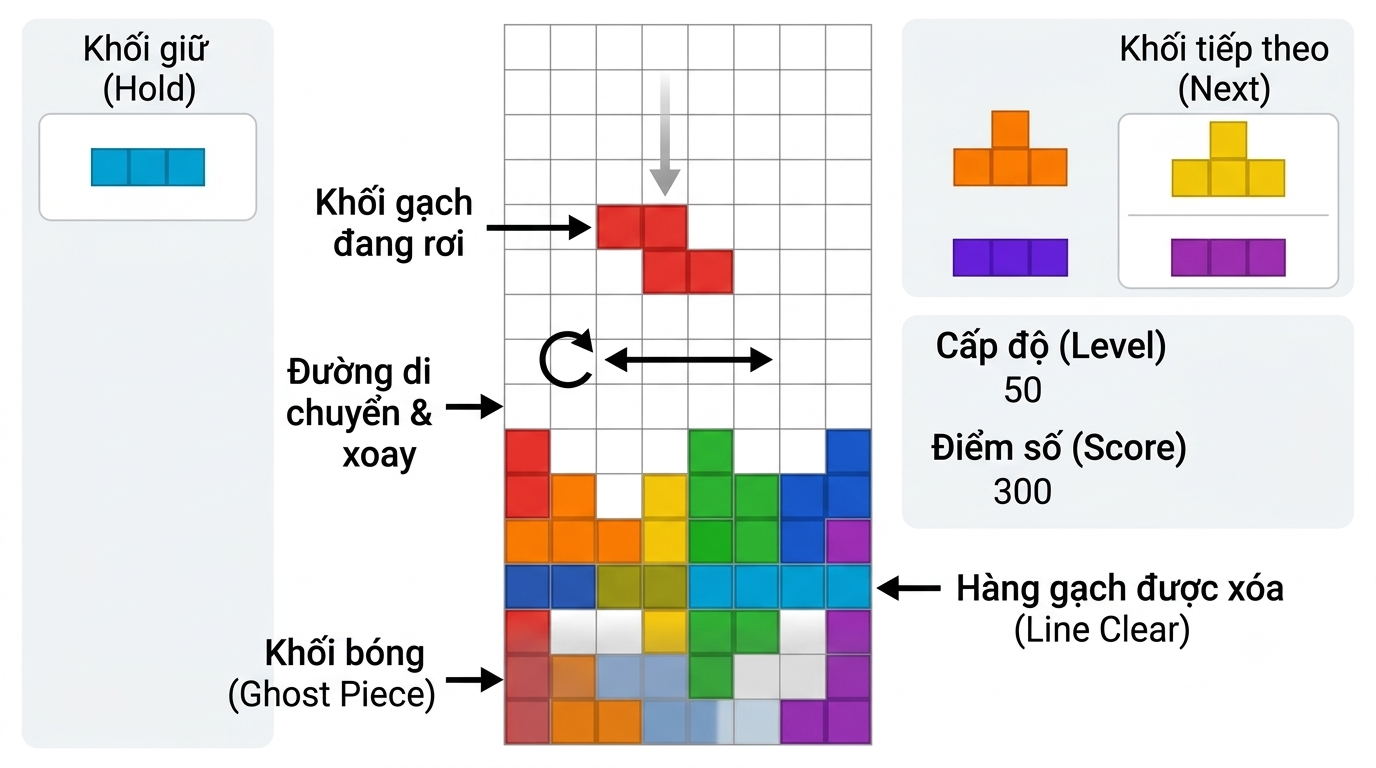
\includegraphics[width=0.75\textwidth]{imgs/chuc_nang_game.png}
    \caption{Sơ đồ minh họa các chức năng và cơ chế hoạt động chính của game Tetris}
    \label{fig:cac_chuc_nang}
\end{figure}

\subsection{Hệ thống tương tác và điều khiển khối (Block Manipulation)}
\begin{itemize}
    \item \textbf{Di chuyển ngang:} Cho phép dịch chuyển khối sang trái hoặc phải theo từng ô vuông hoặc di chuyển liên tục khi giữ phím.
    \item \textbf{Xoay khối (Super Rotation System - SRS):} Cho phép xoay khối $90^\circ$ theo chiều kim đồng hồ hoặc ngược chiều kim đồng hồ, tích hợp cơ chế xử lý va chạm (\textit{Wall Kick}) giúp khối xoay linh hoạt ngay cả khi sát tường~\cite{tetris_guideline}.
    \item \textbf{Rơi chậm (Soft Drop) và Rơi nhanh (Hard Drop):} 
    \begin{itemize}
        \item \textit{Soft Drop:} Tăng tốc độ rơi của khối gạch trong khi người chơi giữ phím điều hướng xuống.
        \item \textit{Hard Drop:} Thả khối gạch rơi lập tức xuống vị trí thấp nhất và khóa cố định tại đó.
    \end{itemize}
    \item \textbf{Thời gian trễ khóa (Lock Delay):} Cung cấp một khoảng thời gian ngắn sau khi khối tiếp đất để người chơi tiếp tục điều chỉnh vị trí trước khi khối bị khóa hẳn~\cite{tetris_lock}.
\end{itemize}

\subsection{Các chức năng giao diện hỗ trợ người chơi (UI/UX)}
Như được minh họa ở Hình~\ref{fig:cac_chuc_nang}, giao diện trò chơi cung cấp các tính năng bổ trợ quan trọng:
\begin{itemize}
    \item \textbf{Xem trước khối tiếp theo (Next Piece Preview):} Hiển thị khối gạch sắp xuất hiện ở bảng phụ bên cạnh, giúp người chơi chủ động tính toán chiến thuật.
    \item \textbf{Cất giữ khối (Hold Piece):} Cho phép tạm lưu khối gạch hiện tại vào ô dự trữ và đổi lấy khối khác khi cần. Mỗi khối mới chỉ được thực hiện thao tác cất giữ tối đa 1 lần.
    \item \textbf{Khối bóng gợi ý (Ghost Piece):} Hiển thị bóng mờ của khối gạch ở đáy lưới, giúp xác định chính xác vị trí khối sẽ đáp xuống.
\end{itemize}

\subsection{Xử lý xóa hàng, tính điểm và tăng cấp độ}
\begin{itemize}
    \item \textbf{Xóa hàng và Tính điểm:} Khi một hàng ngang được lấp đầy 10 ô gạch, hàng đó sẽ tự động biến mất và các khối phía trên dời xuống. Hệ thống thưởng điểm cao hơn khi xóa nhiều hàng cùng lúc (Single, Double, Triple, Tetris) hoặc thực hiện các chuỗi xóa liên tiếp (\textit{Combo}, \textit{Back-to-Back})~\cite{tetris_scoring}.
    \item \textbf{Tăng cấp độ (Level Progression):} Tốc độ rơi của khối tăng dần theo cấp độ (hoặc sau mỗi 10 hàng xóa được), tạo ra độ khó và áp lực thời gian tăng dần~\cite{tetris_marathon}.
    \item \textbf{Kết thúc trò chơi (Game Over / Top Out):} Trò chơi dừng lại và thông báo kết thúc khi khối gạch mới bị chồng lấn hoặc không thể xuất hiện thêm trong vùng chơi~\cite{tetris_topout}.
\end{itemize}


% --------------------------------------------------------------------
%  CHƯƠNG 3 -- Đánh giá thực hiện hợp đồng nhóm
% --------------------------------------------------------------------
\chapter{Đánh giá thực hiện hợp đồng nhóm}

% Điền mức đánh giá theo bảng tiêu chí ở mục \ref{sec:tieu_chi} (Xuất sắc / Tốt / Đạt / Chưa đạt)
\begin{table}[H]
\centering
\small
\caption{Đánh giá các thành viên}\label{tab:danh_gia_thanh_vien}
\renewcommand{\arraystretch}{1.6}
\begin{tabular}{|>{\raggedright\arraybackslash}p{2.6cm}|*{5}{>{\centering\arraybackslash}p{2.1cm}|}}
\hline
\textbf{Tiêu chí} & \textbf{Nguyễn Thịnh} & \textbf{Nguyễn Việt Lâm} & \textbf{Trương Tấn Phát} & \textbf{Thái Trí Nhân} & \textbf{Võ Ngọc Thơ} \\ \hline
Thái độ           & Tốt & Tốt & Tốt & Tốt & Tốt \\ \hline
Đóng góp          & Tốt & Tốt & Tốt & Tốt & Tốt \\ \hline
Quản lý thời gian & Tốt & Tốt & Tốt & Tốt & Tốt \\ \hline
Đóng góp ý kiến   & Tốt & Tốt & Tốt & Tốt & Tốt \\ \hline
Làm việc nhóm     & Tốt & Tốt & Tốt & Tốt & Tốt \\ \hline
\end{tabular}
\end{table}

% =========================== TÀI LIỆU THAM KHẢO =====================
\begin{thebibliography}{99}
\addcontentsline{toc}{chapter}{NGUỒN THAM KHẢO}
\small
% Các \bibitem phần giới thiệu, được \input trong thebibliography ở main.tex
% Người viết: Nguyễn Việt Lâm

\bibitem{tetris_wiki} Wikipedia, ``Tetris'' (truy cập ngày 08/11/2026).
\\\url{https://en.wikipedia.org/wiki/Tetris} 

\bibitem{guardian_tetris} A. Pajitnov, ``How we made Tetris'', \textit{The Guardian}, 02/06/2014.\\ \url{https://www.theguardian.com/culture/2014/jun/02/how-we-made-tetris}

\bibitem{filfre_tetris} J. Maher, ``A Tale of the Mirror World, Part 3: A Game of Falling Shapes'', \textit{The Digital Antiquarian}, 30/06/2017.\\
\url{https://www.filfre.net/2017/06/a-tale-of-the-mirror-world-part-3-a-game-of-falling-shapes}

\bibitem{denofgeek_tetris} Den of Geek, ``Tetris: 10 Facts You Need to Know About the Game's History''.\\ 
\url{https://www.denofgeek.com/games/tetris-game-weird-history}

\bibitem{tetris_myjoy} MyJoyOnline, ``Tetris: the Soviet mind game that took over the world''.\\ 
\url{https://www.myjoyonline.com/tetris-the-soviet-mind-game-that-took-over-the-world/}

% Các \bibitem phần cách chơi, được \input trong thebibliography ở main.tex
% Người viết: Thái Trí Nhân

\bibitem{tetris_official}
Tetris, ``Tetris - Marathon'', Tetris.com
(truy cập ngày 11/11/2026).\\
\url{https://play.tetris.com/games/marathon/}

\bibitem{tetris_guideline}
Tetris Wiki, ``Tetris Guideline''
(truy cập ngày 11/11/2026).\\
\url{https://tetris.wiki/Tetris_Guideline}

\bibitem{tetris_scoring}
Tetris Wiki, ``Scoring''
(truy cập ngày 11/11/2026).\\
\url{https://tetris.wiki/Scoring}

\bibitem{tetris_randomizer}
Tetris Wiki, ``Random Generator''
(truy cập ngày 11/11/2026).\\
\url{https://tetris.wiki/Random_Generator}

\bibitem{tetris_lock}
Tetris Wiki, ``Lock delay''
(truy cập ngày 11/11/2026).\\
\url{https://tetris.wiki/Lock_delay}

\bibitem{tetris_topout}
Tetris Wiki, ``Top out''
(truy cập ngày 11/11/2026).\\
\url{https://tetris.wiki/Top_out}

% Các \bibitem phần chức năng chính, được \input trong thebibliography ở main.tex
% Người viết: Võ Ngọc Thơ

\bibitem{tetris_marathon}
Tetris Wiki, ``Marathon''
(truy cập ngày 11/11/2026).\\
\url{https://tetris.wiki/Marathon}


\end{thebibliography}

\end{document}
